\documentclass{article}
\usepackage[utf8]{inputenc}

\title{Informe del parcial 1}
\author{Jackh Emmanuel Narvaez Guerra, Jeisson Arley Alvarez Giraldo, Miguel Angel Alvarez}
\date{April 2021}

\usepackage{natbib}
\usepackage{graphicx}

\begin{document}

\maketitle

\section{Detalles del desarrollo}
nuestra primer idea fue empezar por el desarrollo en el tinkercard idealizando que tendriamos que hacer un circuito en paralelo para poder darle la opcion de encender uno o mas bombillos ya que si fuera en serie si no se prende uno entonces ninguno prende, ya en el transcurso de que fuimos imaginando como seria plantando las ideas de usar transistores y calculando el promedio de las resistencias las ideas empezaron a fluir por si solas, tenemos pensado utiliza matrices y apuntadores para la implementacion del algoritmo en el momento solo es una idea mientras que analizamos bien las situaciones que se puedan presentar en el proceso, tambien creamos el GitHub y nos aseguramos que si pueda ser modificado por cualquiera de nuestros compañeros tuvimos un percanse que uno de los compañeros no tenia el GitHub Destokp y no nos permitia modificar 
-los circuitos en serie no importa si la resistencia la pone por el lado positivo o negativo, se le es indiferente 

\begin{figure}[h!]
\centering
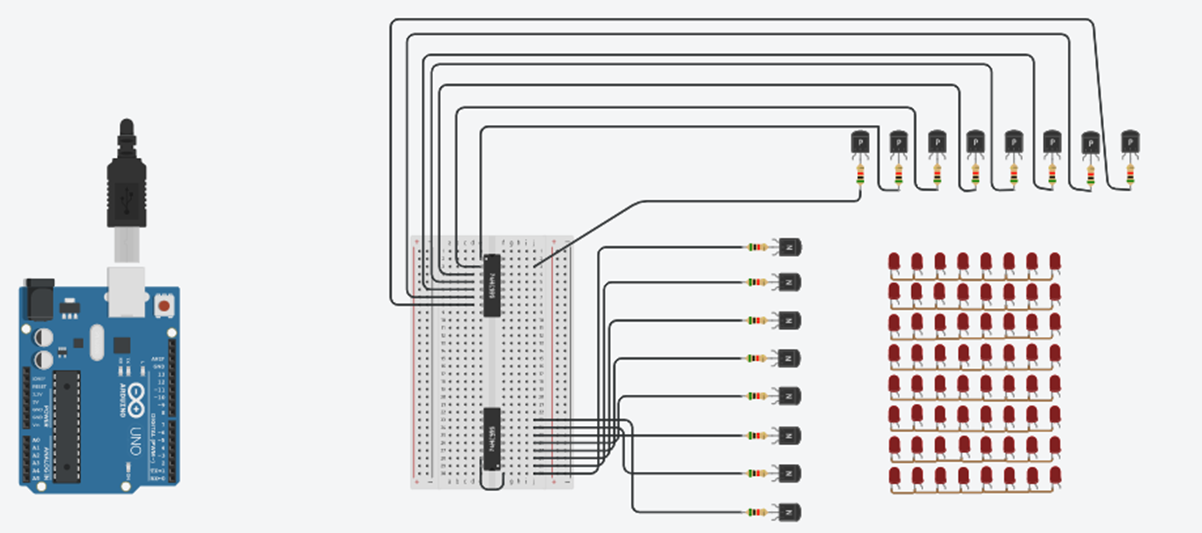
\includegraphics[scale=1.7]{imagen.png}
\caption{The Universe}
\label{fig:universe}
\end{figure}


\section{problemas del desarrollo}
problema1: tuvimos problemas con los transitores, el P funcionaba perfectamente mientras en N tuvimos dudas ya que el P recibe 0 y el N recibe 1, lo cual nos llevo a preguntarnos si se debia a eso
problema2: tuvimos una duda respecto a si se podia usar transistores lo que nos llevo a reiniciar todas las ideas ya propuestas, las resistencias las vamos a empezar a trabajar en 220 omnos
\section{Conclusion}
``I always thought something was fundamentally wrong with the universe'' \citep{adams1995hitchhiker}

\bibliographystyle{plain}
\bibliography{references}
\end{document}
